% Supplementary Material: Filtered Plots
% Derivative Estimation Benchmark Study
\documentclass[11pt]{article}

\usepackage[utf8]{inputenc}
\usepackage[T1]{fontenc}
\usepackage{amsmath,amssymb}
\usepackage{graphicx}
\usepackage[margin=0.75in]{geometry}
\usepackage{hyperref}

\hypersetup{
    colorlinks=true,
    linkcolor=blue,
    citecolor=blue,
    urlcolor=blue,
}

\graphicspath{{paper_figures/supplementary/}}

\title{Supplementary Material: Filtered Performance Plots\\
Derivative Estimation Benchmark Study}
\author{Visual Analysis with Outlier Filtering}
\date{\today}

\begin{document}

\maketitle

\section*{Overview}

This document presents filtered visualizations of method performance across derivative orders and noise levels. All plots use nRMSE capping/filtering to prevent extreme outliers from obscuring meaningful comparisons.

\textbf{Filtering approach:}
\begin{itemize}
    \item Heatmaps: nRMSE values capped at 2.0--10.0 depending on visualization
    \item Line plots: nRMSE capped at 10.0 to show trends without catastrophic outliers
    \item Methods ranked by filtered average (excluding extreme failures) to identify consistently good performers
\end{itemize}

\textbf{Rationale:} Unfiltered plots are dominated by catastrophic failures (nRMSE $> 10^{10}$), making it impossible to distinguish between methods in the usable range (nRMSE $< 1.0$). Capping preserves ranking information while improving readability.

\clearpage

%==============================================================================
% FIGURE 1: HEATMAP OF TOP METHODS
%==============================================================================

\section{Performance Heatmap: Top Methods Across Orders}

Figure~\ref{fig:heatmap} shows nRMSE for the top 10 methods (by filtered average) across all 8 derivative orders. Each subplot represents a fixed order; rows are methods, columns are noise levels.

\textbf{Key observations:}
\begin{itemize}
    \item GP methods (top 4 rows) show consistent performance across all orders
    \item Fourier-Interp (row 5) maintains good performance at high orders
    \item AAA methods (bottom rows) show degradation at orders $\geq 3$
    \item Color gradient reveals smooth vs abrupt failure modes
\end{itemize}

\begin{figure}[p]
\centering
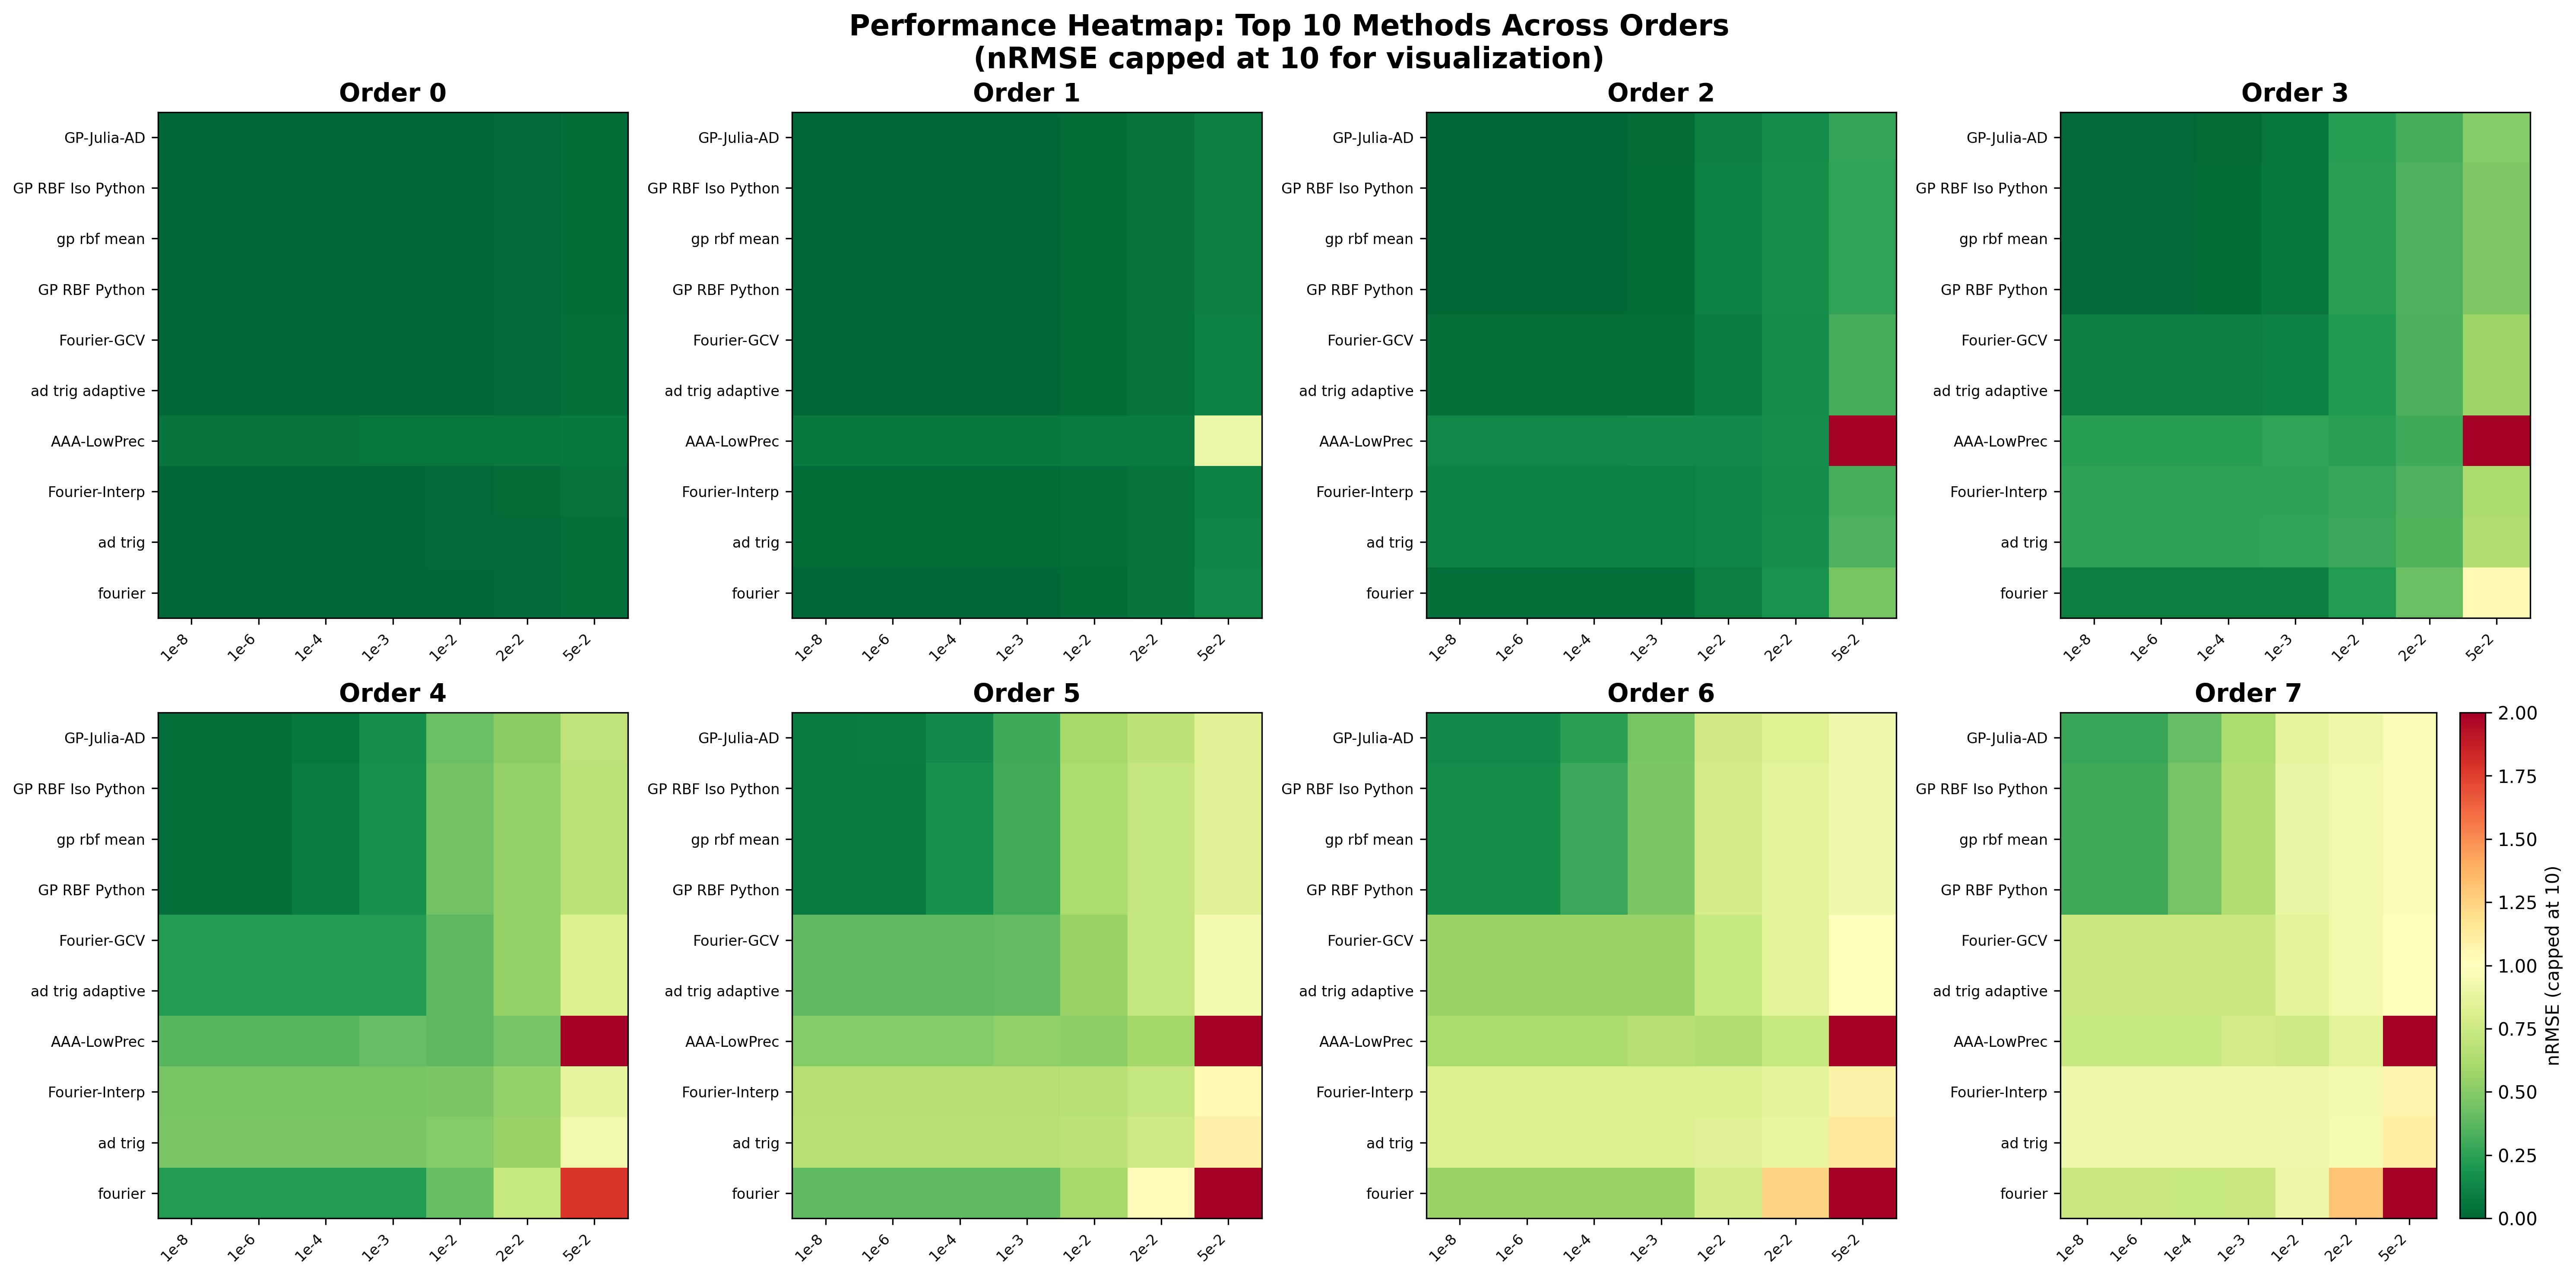
\includegraphics[width=\textwidth]{heatmap_top_methods.png}
\caption{Performance heatmap for top 10 methods across derivative orders. nRMSE values capped at 10 for visualization. Color scale: green (excellent) to red (poor).}
\label{fig:heatmap}
\end{figure}

\clearpage

%==============================================================================
% FIGURE 2: NOISE SENSITIVITY
%==============================================================================

\section{Noise Sensitivity Analysis}

Figure~\ref{fig:noise_sensitivity} shows nRMSE vs noise level for the top 5 methods at each derivative order. Horizontal dashed line at nRMSE = 1.0 indicates transition to poor performance.

\textbf{Key observations:}
\begin{itemize}
    \item At low orders (0--2), most methods show flat or gently increasing curves
    \item At high orders (5--7), curves become steeper---noise amplification dominates
    \item GP methods maintain relatively flat curves even at high orders (robust)
    \item Crossing points reveal order-dependent method rankings
\end{itemize}

\begin{figure}[p]
\centering
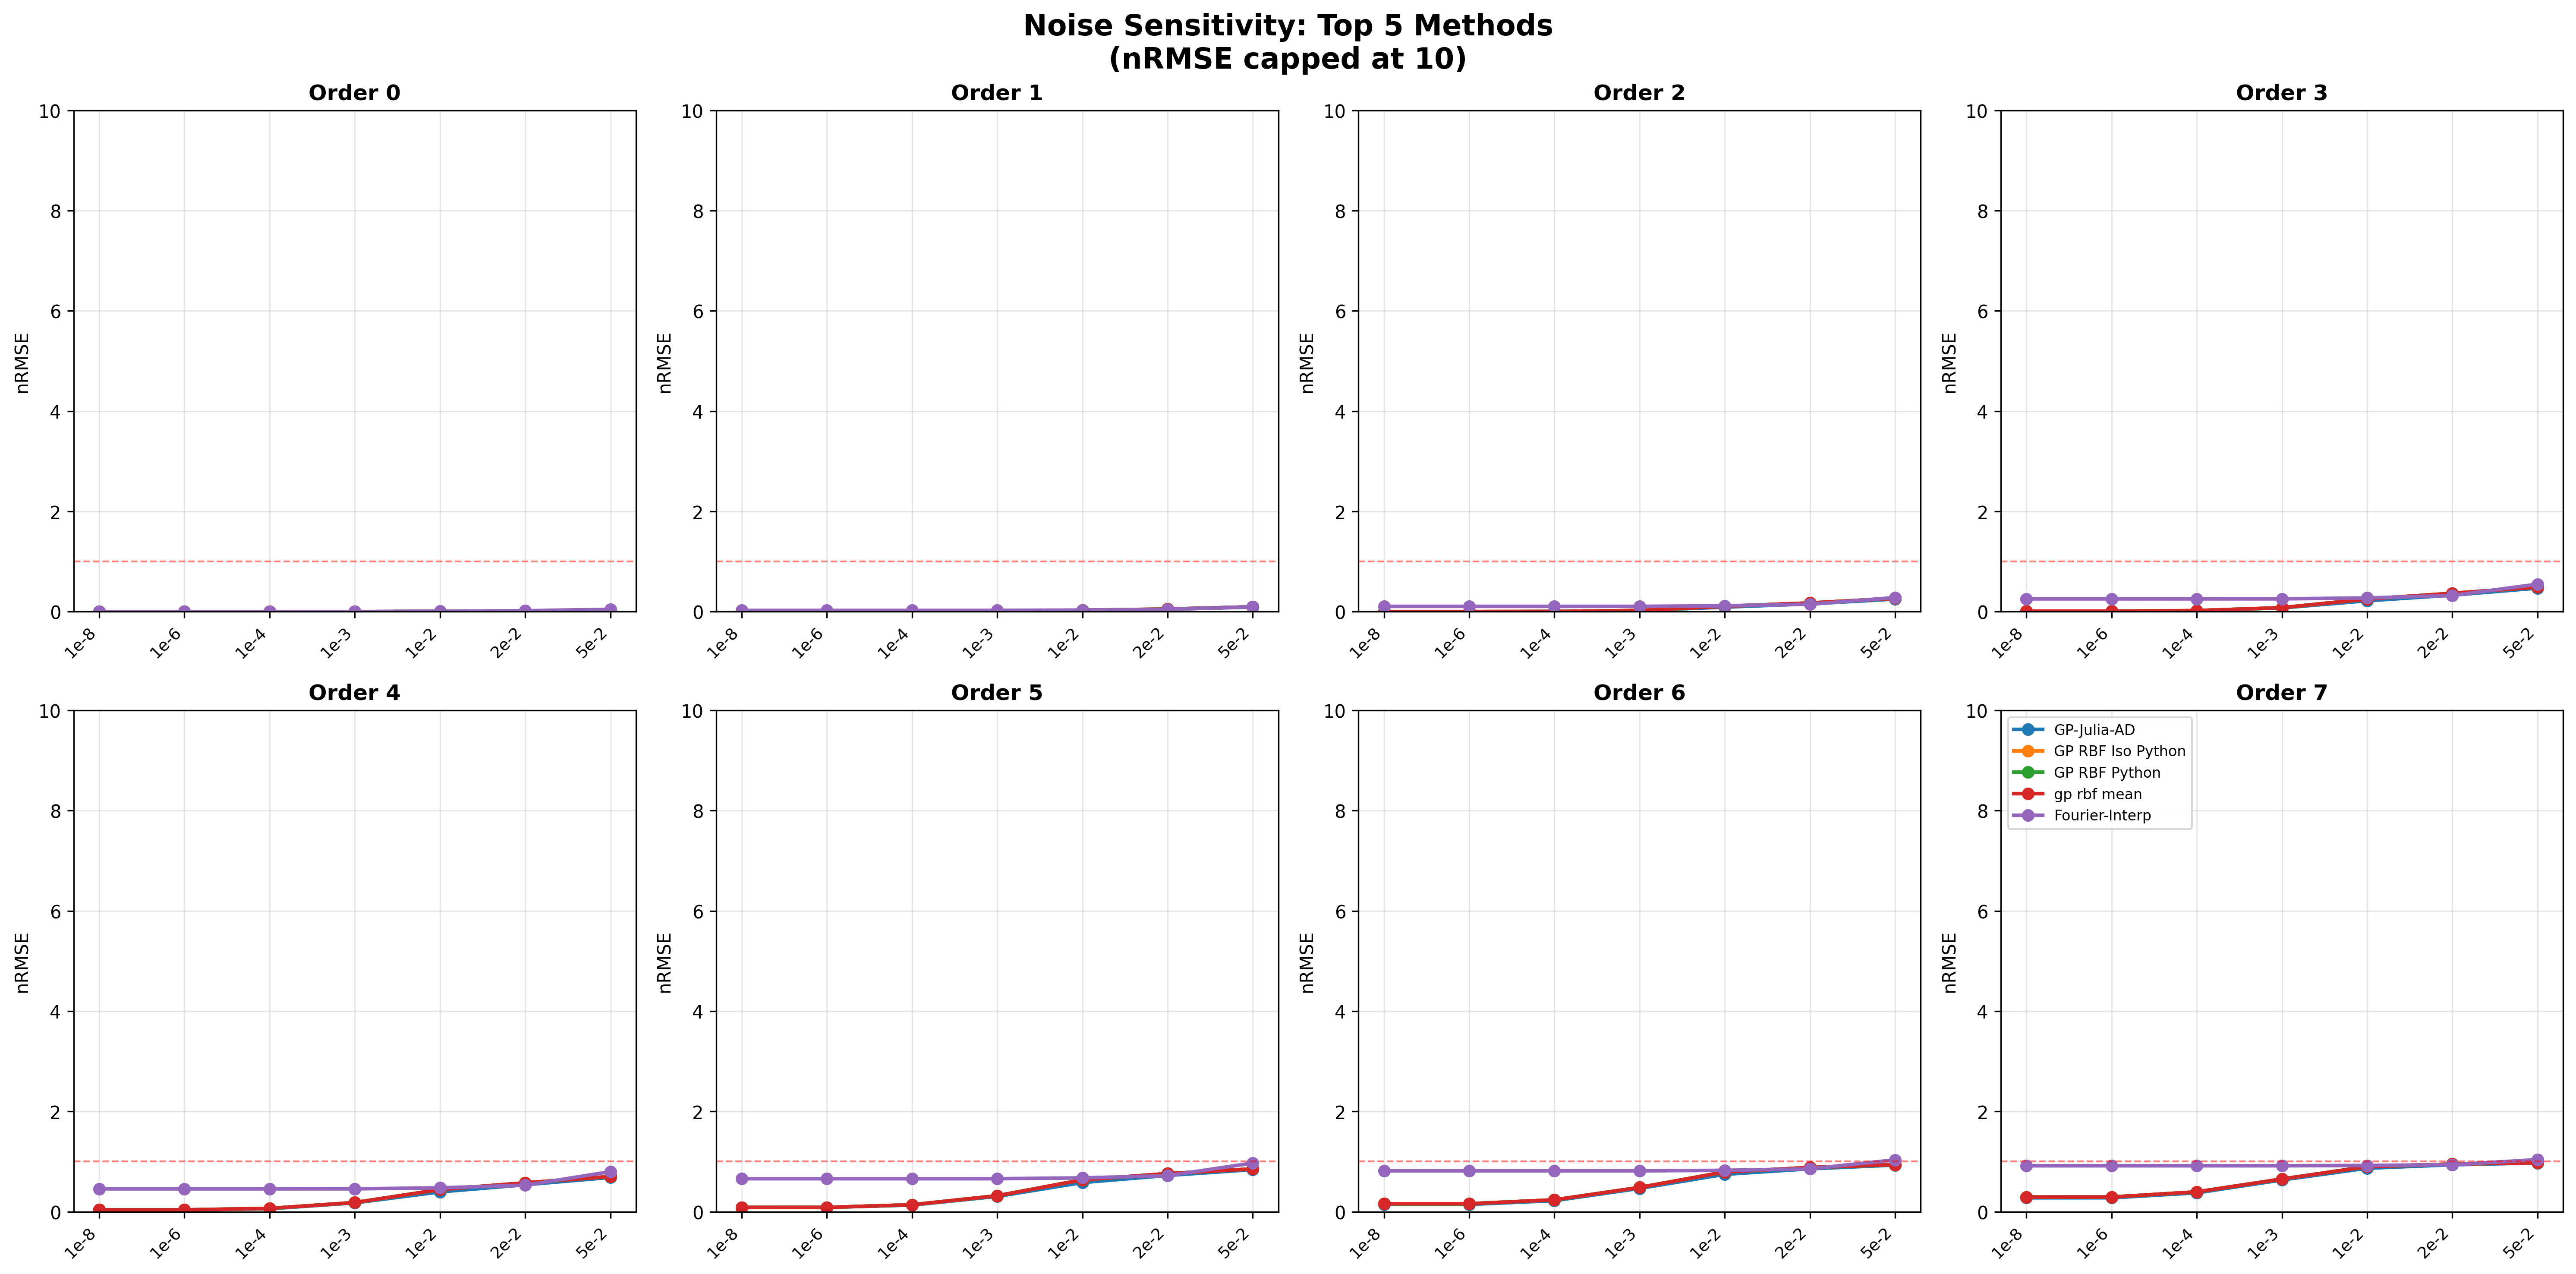
\includegraphics[width=\textwidth]{noise_sensitivity_top5.png}
\caption{Noise sensitivity curves for top 5 methods across all derivative orders. nRMSE capped at 10. Red dashed line indicates nRMSE = 1.0 threshold.}
\label{fig:noise_sensitivity}
\end{figure}

\clearpage

%==============================================================================
% FIGURE 3: ORDER PROGRESSION
%==============================================================================

\section{Order Progression at Moderate Noise}

Figure~\ref{fig:order_progression} shows how nRMSE changes with derivative order for the top 5 methods at noise level $10^{-3}$ (moderate noise regime).

\textbf{Key observations:}
\begin{itemize}
    \item All methods show monotonic increase with order (expected from noise amplification theory)
    \item GP-Julia-AD exhibits slowest growth rate---most robust to high-order differentiation
    \item Fourier-Interp shows competitive performance despite spectral noise amplification
    \item AAA-HighPrec absent from top 5 due to catastrophic failure at orders $\geq 3$
\end{itemize}

\textbf{Interpretation:} Slope of curves indicates noise amplification factor. Shallower slope = better regularization/noise handling.

\begin{figure}[p]
\centering
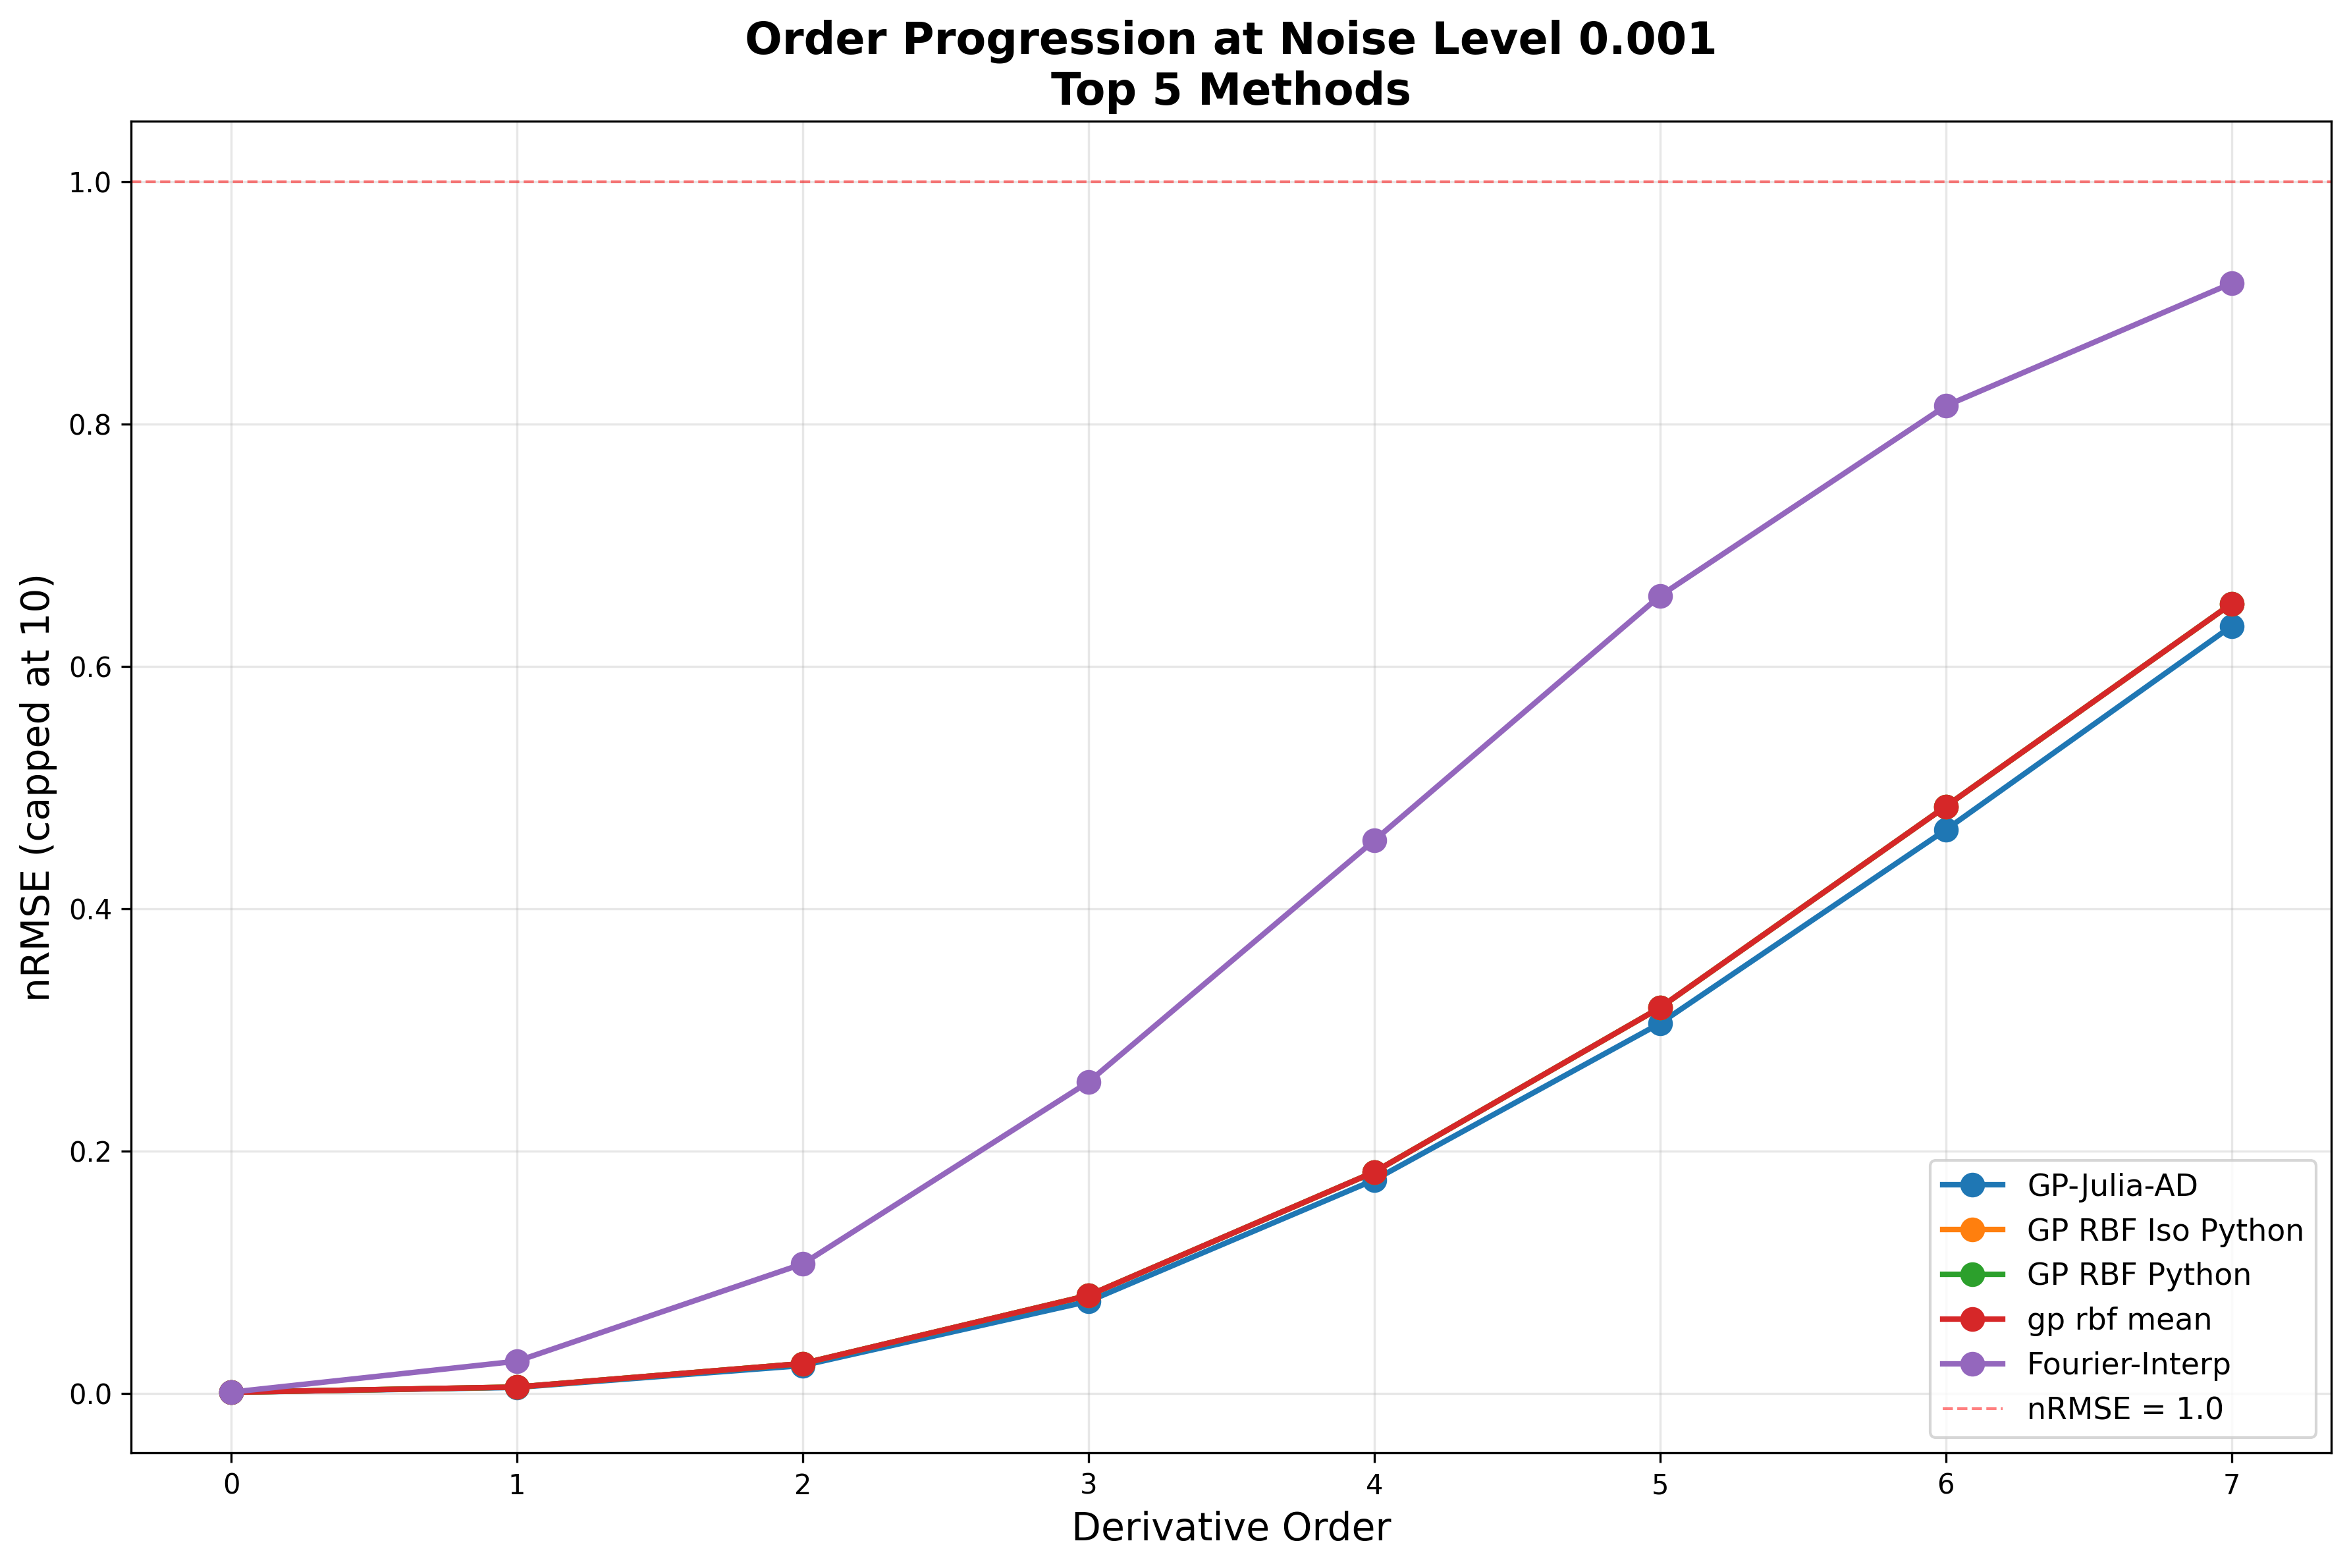
\includegraphics[width=0.9\textwidth]{order_progression_moderate_noise.png}
\caption{Order progression for top 5 methods at noise level $10^{-3}$. nRMSE capped at 10. Red dashed line indicates nRMSE = 1.0 threshold.}
\label{fig:order_progression}
\end{figure}

\clearpage

%==============================================================================
% FIGURE 4: PER-METHOD HEATMAPS
%==============================================================================

\section{Per-Method Performance Profiles}

Figure~\ref{fig:per_method} shows complete performance profiles (noise $\times$ order) for the top 6 methods. Each subplot is a 2D heatmap with noise levels as rows and derivative orders as columns.

\textbf{Key observations:}
\begin{itemize}
    \item GP methods (subplots 1--4): Gradual color gradient from green to yellow---graceful degradation
    \item Fourier-Interp (subplot 5): Vertical banding visible---order-dependent performance
    \item AAA methods show abrupt color transitions at order 3---catastrophic failure boundary
\end{itemize}

\textbf{Use case:} Quickly assess if a specific method is suitable for your (order, noise) operating point by checking the corresponding cell color.

\begin{figure}[p]
\centering
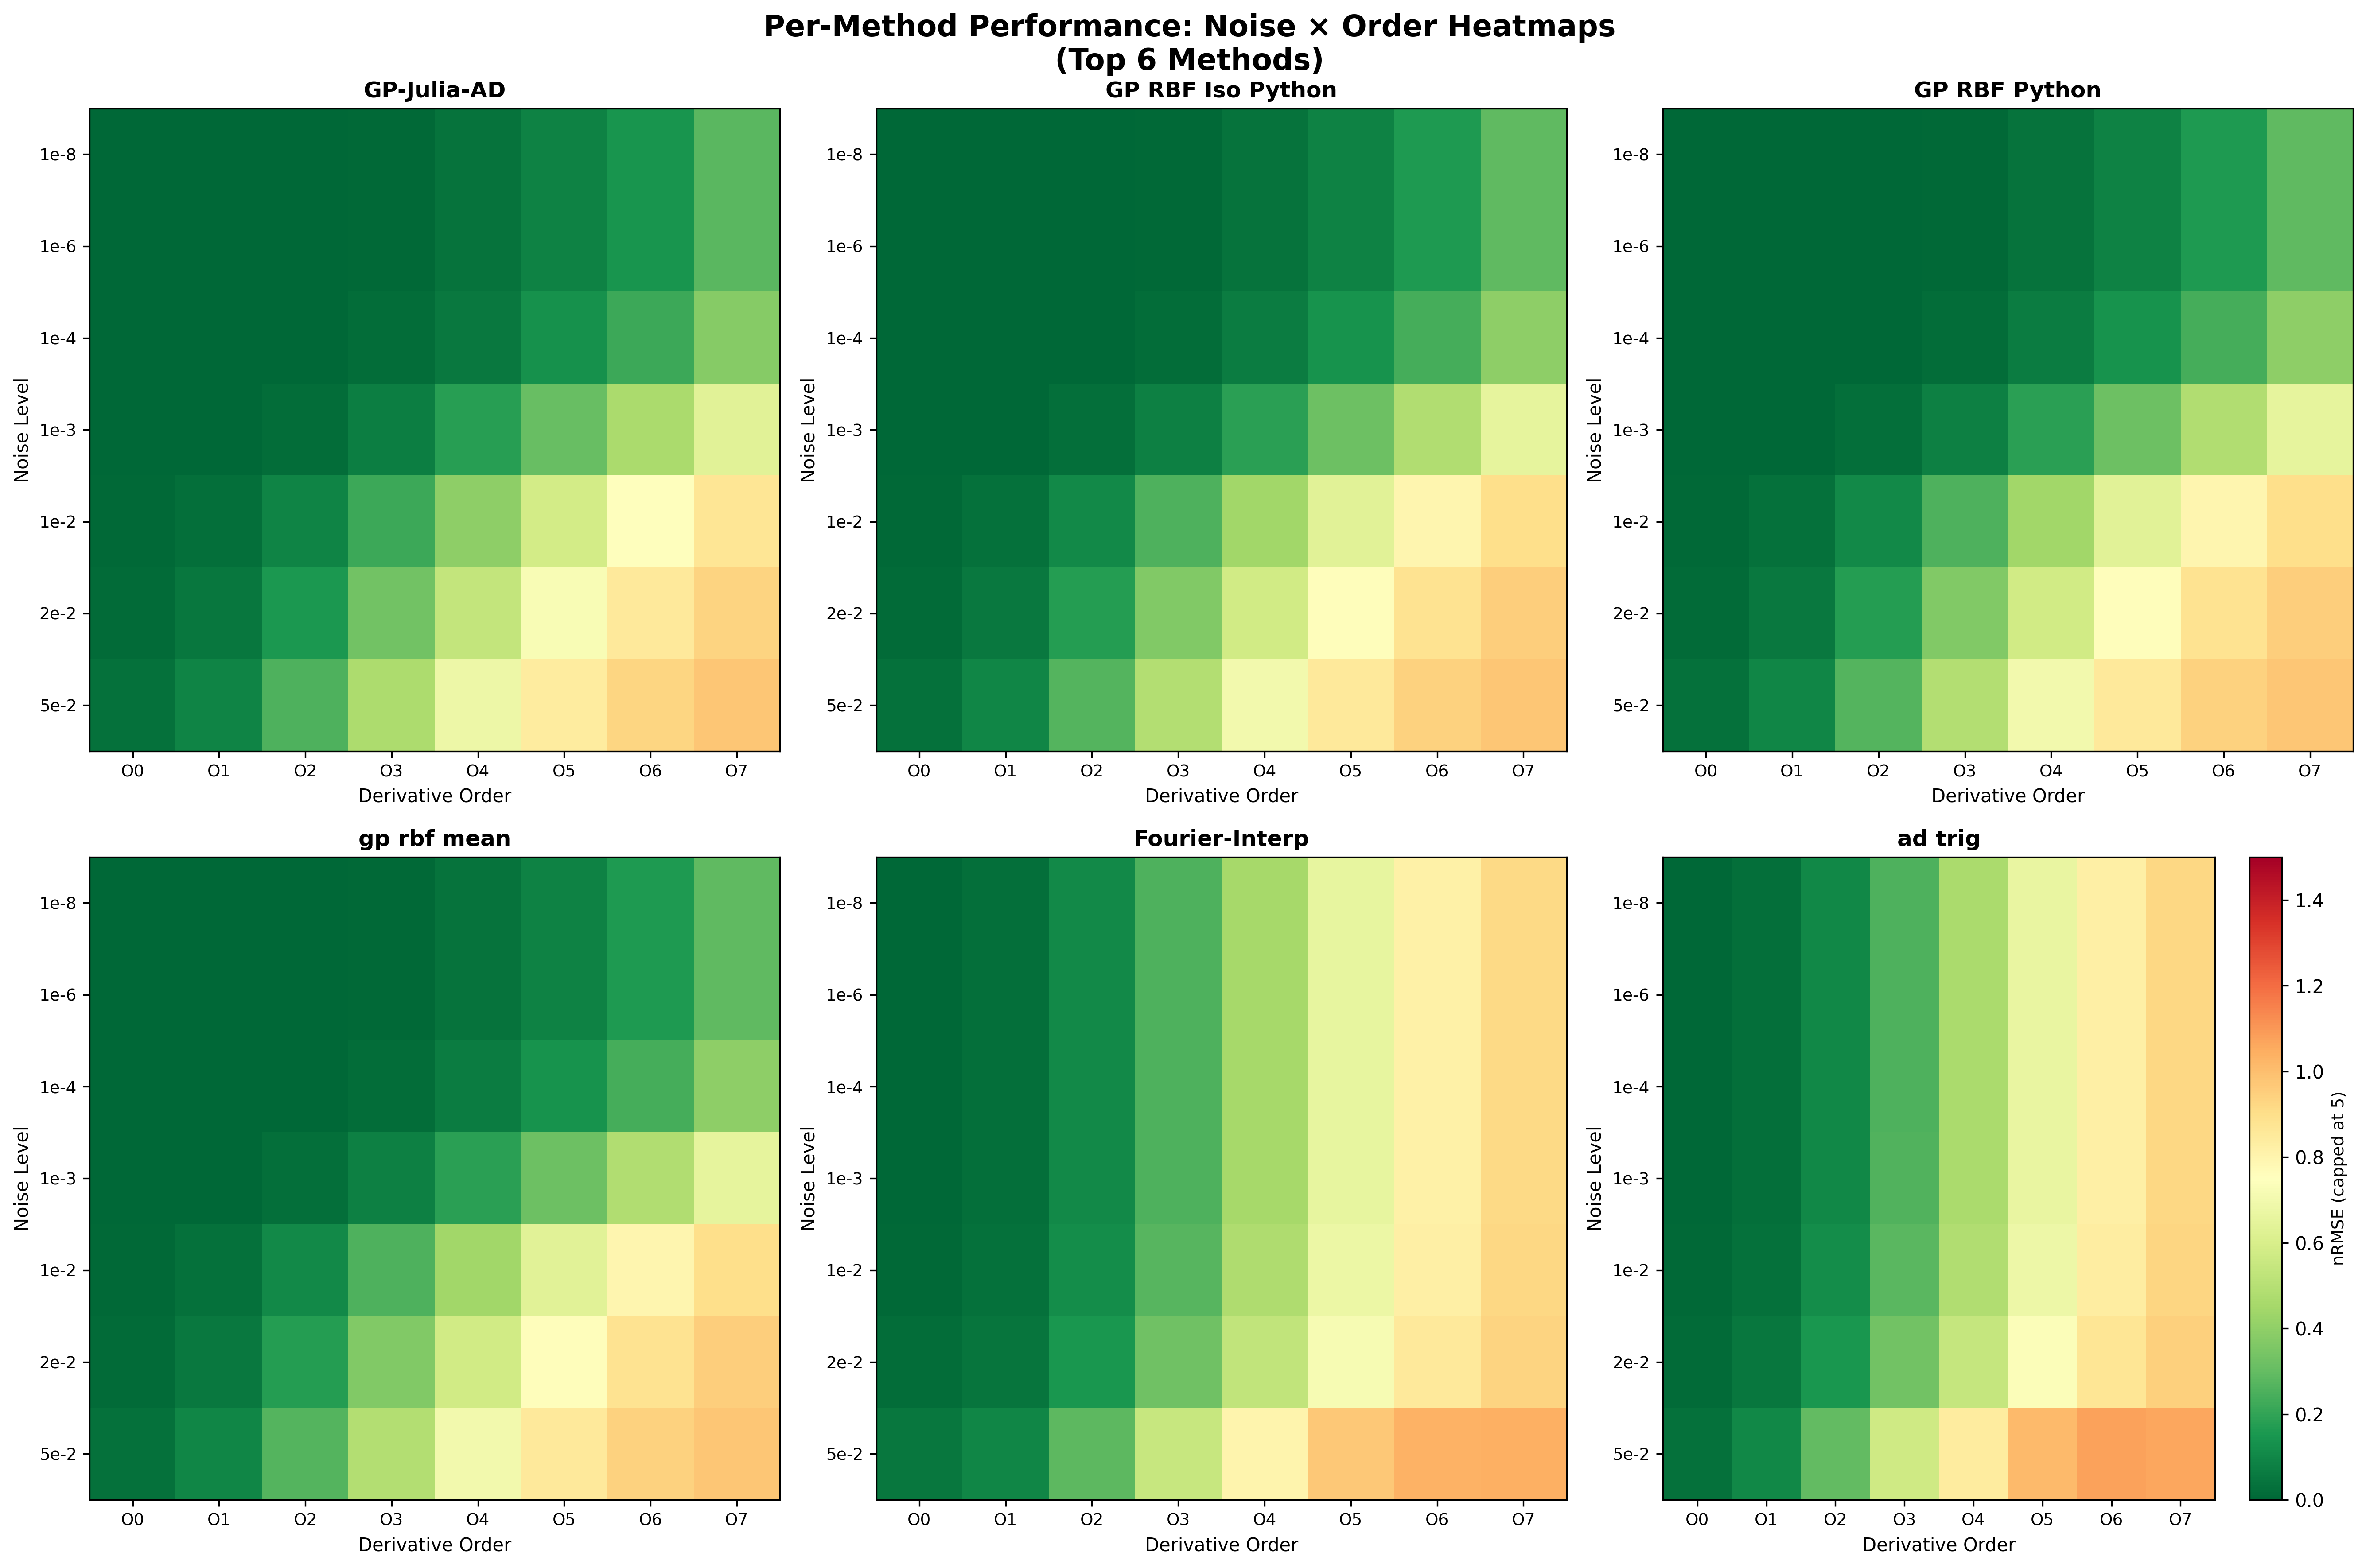
\includegraphics[width=\textwidth]{per_method_heatmaps.png}
\caption{Per-method heatmaps showing nRMSE across all noise levels and derivative orders. nRMSE capped at 5 for better visualization of non-catastrophic behavior. Color scale consistent across subplots.}
\label{fig:per_method}
\end{figure}

\clearpage

%==============================================================================
% SUMMARY
%==============================================================================

\section*{Summary}

These filtered plots complement the detailed tables (see supplementary\_data\_tables\_final.pdf) by providing visual confirmation of:

\begin{enumerate}
    \item \textbf{Method stratification:} Clear visual separation between robust (GP), competitive (Fourier), and fragile (AAA) methods
    \item \textbf{Noise amplification scaling:} Exponential growth in nRMSE with order visible in all plots
    \item \textbf{Coverage gaps:} Missing data points (gaps in line plots) indicate method scope limitations
    \item \textbf{Failure modes:} Abrupt vs gradual degradation patterns distinguishable by color transitions
\end{enumerate}

\textbf{Filtering impact:} By capping nRMSE at 10, we lose information about the \emph{magnitude} of catastrophic failures (e.g., AAA at order 7: nRMSE $\approx 10^{10}$) but gain ability to compare methods in the usable range. Refer to detailed tables for uncapped values.

\textbf{Data source:} All plots generated from comprehensive\_summary.csv (1,310 experimental data points, 3 trials each).

\end{document}
